\chapter{Lec 04 - 05 - Statistical Learning}

\maketitle

\section{What Is Statistical Learning?}
In order to motivate our study of statistical learning, we begin with a simple example. Suppose that we are statistical consultants hired by a client to provide advice on how to improve sales of a particular product. The Advertising data set consists of the sales of that product in 200 different markets, along with advertising budgets for the product in each of those markets for three different media: TV, radio, and newspaper.\\\\
In this setting, the advertising budgets are \textit{input} variables while sales is an \textit{output} variable. The input variables are typically denoted using the symbol $X$, with a subscript to distinguish them. So $X_1$ might be the TV budget, $X_2$ the radio budget, and $X_3$ the newspaper budget. The inputs go by different names, such as \textit{predictors}, \textit{independent variables}, \textit{features}, while the output variable—in this case, sales—is often called the \textit{response}.
\begin{center}
    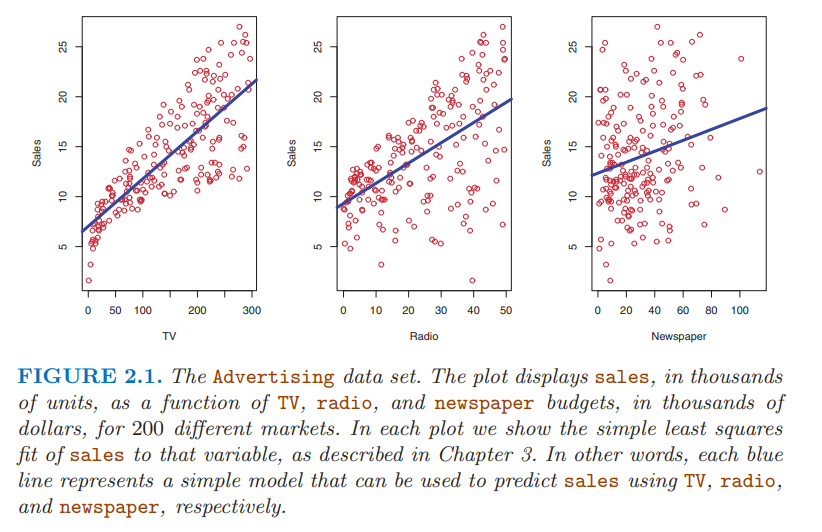
\includegraphics[scale=0.8]{images/tv adv.png}
\end{center}
More generally, suppose that we observe a quantitative response $Y$ and $p$
different predictors, $X_1, X_2,...,X_p$. We assume that there is some
relationship between $Y$ and $X = (X_1, X_2,...,X_p)$, which can be written
in the very general form
\[Y = f(X) + \epsilon\]
Here $f$ is some fixed but \textbf{unknown function} of $X_1,...,X_p$, and $\epsilon$ is a random error term, which is independent of $X$ and has mean zero \footnote{ $\epsilon$ captures measurement errors and other discrepancies}.  In this formulation, $f$ represents the systematic information that $X$ provides about $Y$. In essence, statistical learning refers to a set of approaches for \textbf{estimating}
$f$. 


\section{Prediction}
With a good estimate for $f$ we can make predictions of $Y$ at new points $X = x$. We can predict $Y$ using
\[\hat{Y} = \hat{f}(X)\]
where $\hat{f}$ represents our estimate for $f$, and $\hat{Y}$ represents the resulting prediction for $Y$. The accuracy of $\hat{Y}$ as a prediction for $Y$ depends on two quantities, which we will call the \textit{reducible error} and the \textit{irreducible error}. In general, $\hat{f}$ will not be a perfect estimate for $f$, and this inaccuracy will introduce some error. This error is reducible because we can potentially improve the
accuracy of $\hat{f}$ by using the most appropriate statistical learning technique to estimate $f$. However, even if it were possible to form a perfect estimate for $f$, our prediction would still have some error in it! This is because $Y$ is also a function of
$\epsilon$, which, by definition, cannot be predicted using $X$. Therefore, variability
associated with $\epsilon$ also affects the accuracy of our predictions. This is known
as the irreducible error.\\\\
Consider a given estimate $\hat{f}$ and a set of predictors $X$, which yields the prediction $\hat{Y} = \hat{f(X)}$. Assume for a moment that both $\hat{f}$ and $X$ are fixed. Then, it is easy to show that
\begin{center}
    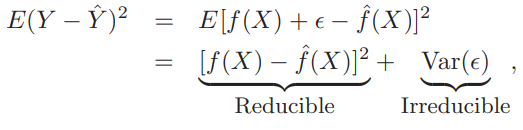
\includegraphics[scale=0.5]{images/formula.png}
\end{center}
where $E(Y - \hat{Y})^2$ represents the average, or expected value, of the squared difference between the predicted and actual value of $Y$ , and $Var(\epsilon)$ represents the variance associated with the error term $\epsilon$. 

\section{How to estimate \textit{f}: Nearest neighbor averaging}
One of the simplest methods to estimate $f$ is to compute the mean over all observations for a given $X$:
\[\hat{f}(x) = E(Y | X = x)\]
where $E(Y | X = x)$ is the expected value (average) of $Y$ given $X = x$. However, typically we have few or zero data points for an exact $X = x$, so we cannot compute $E(Y|X=x)$. Then, we can reformulate $\hat{f}$ as the average of of all the data points in some neighborhood of $x$ $\mathcal{N}(x)$:
\[\hat{f}(x) = \text{Ave}(Y | X \in \mathcal{N}(x))\]
\textbf{Nearest neighbor averaging} can be pretty good for small $p$ (low-dimensional data), i.e. $p \leq 4$. This decrease in performance as the dimension increases is a common problem for this kind of model, and results from the fact that in higher dimensions there is effectively a reduction in sample size. This is due to the so called \textbf{curse of dimensionality}, that is, the $K$ observations that are nearest to a given test observation $x$ may be very far away from $x$ in $p$-dimensional space when $p$ is large, leading to a very poor prediction of $f(x)$.
\begin{center}
    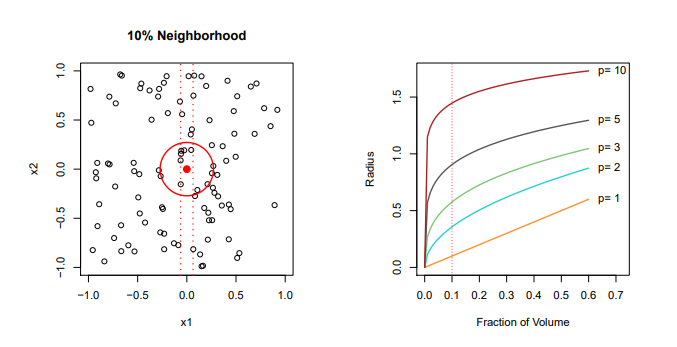
\includegraphics[]{images/curse dimensionality.png}
\end{center}
The concept is that we need to get a reasonable fraction of the $K$ values of $y_i$ to average to bring the variance down, e.g. 10\%. However, A 10\% neighborhood in high dimensions need no longer be local, so we lose the spirit of estimating $E(Y|X=x)$ by local averaging.


\section{Parametric Methods}
Parametric methods involve a two-step model-based approach.
\begin{enumerate}
    \item First, we make an assumption about the functional form, or shape, of $f$. For example, one very simple assumption is that $f$ is linear in $X$: 
    \begin{equation}
        f(X) = \beta_0 + \beta_1 X_1 + \beta_2 X_2 + ... + \beta_p X_p
        \label{linear}
    \end{equation}
    This is a \textbf{linear model}.

    \item After a model has been selected, we need a procedure that uses the training data to \textit{fit} or \textit{train} the model. In the case of the linear model \ref{linear}, we need to estimate the parameters $\beta_0, \beta_1,...,\beta_p$. That is, we want to find values of these parameters such that
    \[Y \approx \beta_0 + \beta_1 X_1 + \beta_2 X_2 + ... + \beta_p X_p\]
\end{enumerate}
The model-based approach just described is referred to as parametric;
it reduces the problem of estimating $f$ down to one of estimating a set of parameters. The potential disadvantage of a parametric approach is that the model we choose will usually not match the true unknown form of $f$.\\\\
A linear model gives a reasonable fit here:
\begin{center}
    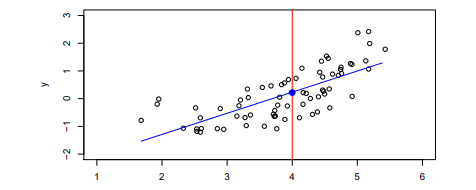
\includegraphics[]{images/linear.png}
\end{center}
A \textbf{quadratic} model $\hat{f}(X) = \beta_0 + \beta_1 X + \beta_2 X^2$ fits slightly better:
\begin{center}
    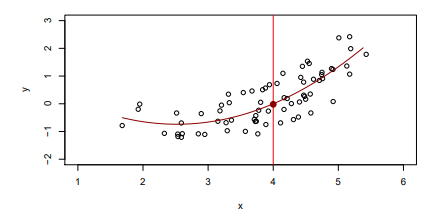
\includegraphics[]{images/quadratic.png}
\end{center}
If the chosen model is too far from the true $f$, then our estimate will be poor. We can try to address this problem by choosing \textit{flexible} models that can fit many different possible functional forms for $f$. But in general, fitting a more flexible model requires estimating a greater number of parameters. These more complex models can lead to a phenomenon known as \textbf{overfitting} the data, which essentially means they model the random noise in the training data, rather than the intended outputs.

\section{Some trade-offs}
Of the many methods that we will examine, some are less flexible, or more restrictive, in the sense that they can produce just a relatively small range of shapes to estimate $f$. For example, the linear regression presented before is a relatively inflexible approach, because it can only generate linear functions. On the other hand, other methods are more flexible.\\\\
One might reasonably ask the following question: \textit{why would we ever
choose to use a more restrictive method instead of a very flexible approach?} There are several reasons that we might prefer a more restrictive model. For example, restrictive models are much more interpretable. In contrast, very flexible approaches can lead to such complicated estimates of $f$ that it is difficult to understand how any individual predictor is associated with the response.\\\\
The figure below provides an illustration of the trade-off between flexibility and interpretability for some methods:
\begin{center}
    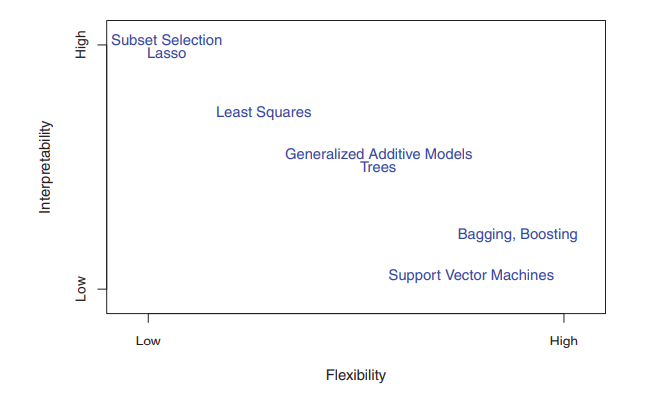
\includegraphics[scale=0.8]{images/trade-off.png}
\end{center}

\section{Assessing Model Accuracy}
In order to evaluate the performance of a statistical learning method on a given data set, we need some way to measure how well its predictions actually match the observed data. In the regression setting, the most commonly-used measure is the \textbf{mean squared error} (MSE), given by
\begin{equation}
    MSE_{Tr} = \frac{1}{n} \sum_{i=1}^n (y_i - \hat{f}(x_i))^2
    \label{MSE}
\end{equation}
The $MSE_{Tr}$ is computed using the training data that was used to fit the model, and so should more accurately be referred to as the training $MSE$. But in general, we do not really care how well the method works on the training data. Rather, we are interested in \textit{the accuracy of the predictions that we obtain when we apply our method to previously unseen test data}.\\\\
How can we go about trying to select a method that minimizes the test
$MSE_{Te}$?  In some settings, we may have a test data set available, that is,
we may have access to a set of observations that were not used to train
the statistical learning method. We can then simply evaluate \ref{MSE} on the
test observations, and select the learning method for which the test $MSE_{Te}$ is smallest. But what if no test observations are available? In that case, one might imagine simply selecting a statistical learning method that minimizes the training $MSE_{Tr}$. Unfortunately, there is a fundamental problem with this strategy: there is no guarantee that the method with the lowest training $MSE_{Tr}$ will also have the lowest test $MSE_{Te}$. The figure below illustrates this phenomenon on a simple example:
\begin{center}
    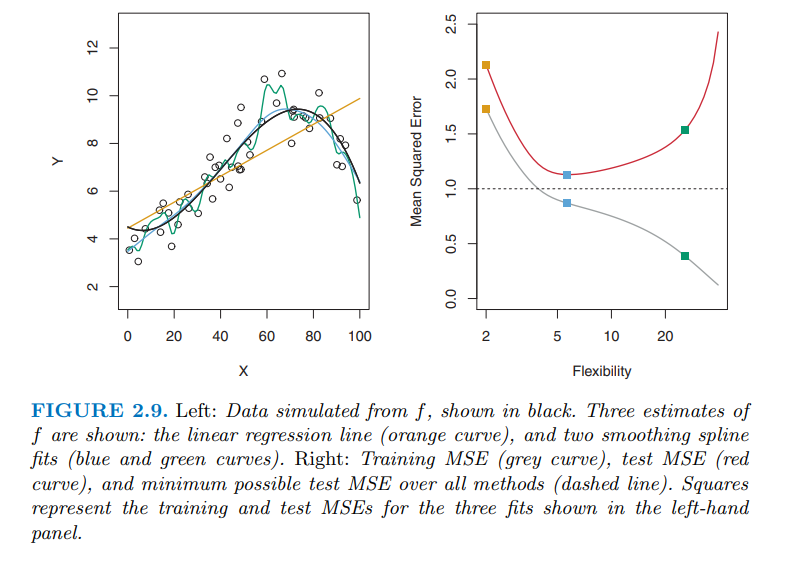
\includegraphics[scale=0.8]{images/overfit_1.png}
\end{center}
As model flexibility increases, training $MSE_{Tr}$ will decrease, but the test $MSE_{Te}$ may not. When a given method yields a small training $MSE_{Tr}$ but a large test $MSE_{Te}$, we are said to be \textit{overfitting} the data. This happens because our statistical learning procedure is working too hard to find patterns in the training data, and may be picking up some patterns that are just caused by random chance rather than by true properties of the unknown function $f$.
\begin{center}
    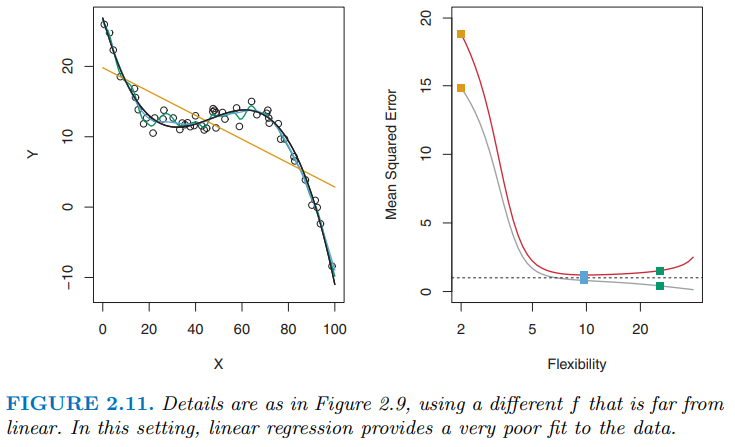
\includegraphics[scale=0.8]{images/overfit_2.png}
\end{center}
The figure above displays an example in which $f$ is highly non-linear. The
training and test $MSE_{Tr}$ curves still exhibit the same general patterns, but now there is a rapid decrease in both curves before the test $MSE_{Te}$ starts to increase slowly.\\\\
In practice, one can usually compute the training $MSE_{Tr}$ with relative
ease, but estimating test $MSE_{Te}$ is considerably more difficult because usually no test data are available. We will discuss a variety of approaches that can be used in practice to estimate $MSE_{Te}$. One important method is \textit{cross-validation}, which is a method for estimating test $MSE_{Te}$ using the training data.

\section{Bias-Variance Trade-Off}
It is possible to show that the expected test $MSE_{te}$, for a given value $x_0$, can always be decomposed into the sum of three fundamental quantities:
\begin{itemize}
    \item the variance of $\hat{f}(x_0)$,
    \item the squared bias of $\hat{f}(x_0)$,
    \item and the variance of the error term $\epsilon$
\end{itemize}
\begin{equation}
    E(y_0 - \hat{f}(x_0))^2 = \text{Var}(\hat{f}(x_0)) + [\text{Bias}(\hat{f}(x_0))]^2 + \text{Var}(\epsilon)
    \label{bias-variance}
\end{equation}
Equation \ref{bias-variance} refers to the average test $MSE_{Te}$ that we would obtain if we repeatedly estimated $f$ using a large number of training sets, and tested each at $x_0$.\\\\
Equation \ref{bias-variance}  tells us that in order to minimize the expected test error, we need to select a statistical learning method that simultaneously achieves low variance and low bias. What do we mean by the variance and bias of a statistical learning method?\\\\
Variance refers to the amount by which $\hat{f}$ would change if we estimated it using a different training data set. Ideally, the estimate for $f$ should not vary too much between training sets. However, if a method has high variance, then small changes in the training data can result in large changes in $\hat{f}$. In general, more flexible statistical methods have higher variance.\\\\
On the other hand, bias refers to the error that is introduced by approximating a real-life problem, which may be extremely complicated, by a much simpler model.\\\\
As a general rule, as we use more flexible methods, the variance will increase and the bias will decrease. The relative rate of change of these two quantities determines whether the test MSE increases or decreases. Therefore, we need to choose the flexibility based on average test error amounts to a bias-variance trade-off. As we increase the flexibility of a class of methods, the bias tends to initially decrease faster than the variance increases. Consequently, the expected test $MSE_{Te}$ declines. However, at some point increasing flexibility has little impact on the bias but starts to significantly increase the variance. When this happens the test $MSE_{Te}$ increases following the $U$-shape curve presented in the figures above.
